%%%%%%%%%%%%%%%%%%%%%%%%%%%%%%%%%%%%%%%%%%%%%%%%%%%%%%%%%%%%%%%%%%%%%%%%%%%%%%%%
% Social Network Analysis for Computer Scientists
% Course paper template (modified version of ACM Proceedings template)
% Frank W. Takes (ftakes@liacs.nl)
% http://liacs.leidenuniv.nl/~takesfw/SNACS
%%%%%%%%%%%%%%%%%%%%%%%%%%%%%%%%%%%%%%%%%%%%%%%%%%%%%%%%%%%%%%%%%%%%%%%%%%%%%%%%

% THIS IS SIGPROC-SP.TEX - VERSION 3.1
% WORKS WITH V3.2SP OF ACM_PROC_ARTICLE-SP.CLS
% APRIL 2009
%
% It is an example file showing how to use the 'acm_proc_article-sp.cls' V3.2SP
% LaTeX2e document class file for Conference Proceedings submissions.
% ----------------------------------------------------------------------------------------------------------------
% This .tex file (and associated .cls V3.2SP) *DOES NOT* produce:
%       1) The Permission Statement
%       2) The Conference (location) Info information
%       3) The Copyright Line with ACM data
%       4) Page numbering
% ---------------------------------------------------------------------------------------------------------------
% It is an example which *does* use the .bib file (from which the .bbl file
% is produced).
% REMEMBER HOWEVER: After having produced the .bbl file,
% and prior to final submission,
% you need to 'insert'  your .bbl file into your source .tex file so as to provide
% ONE 'self-contained' source file.
%
% For tracking purposes - this is V3.1SP - APRIL 2009

\documentclass{acm_proc_article-sp}

\usepackage{url}
\usepackage{color}
\usepackage[hidelinks]{hyperref}
\usepackage{color}
\usepackage{graphicx}
\usepackage{booktabs}
\usepackage{amsmath}
\usepackage{array, multirow}
\usepackage{amssymb}
\usepackage{multicol}
\usepackage{graphicx}
\hypersetup{
	bookmarks=true,         % show bookmarks bar?
	unicode=false,          % non-Latin characters in Acrobat’s bookmarks
	pdftoolbar=true,        % show Acrobat’s toolbar?
	pdfmenubar=true,        % show Acrobat’s menu?
	pdffitwindow=false,     % window fit to page when opened
	pdfstartview={FitH},    % fits the width of the page to the window
	pdftitle={My title},    % title
	pdfauthor={Author},     % author
	pdfsubject={Subject},   % subject of the document
	pdfcreator={Creator},   % creator of the document
	pdfproducer={Producer}, % producer of the document
	pdfkeywords={keyword1, key2, key3}, % list of keywords
	pdfnewwindow=true,      % links in new PDF window
	colorlinks=false,       % false: boxed links; true: colored links
	linkcolor=red,          % color of internal links (change box color with linkbordercolor)
	citecolor=green,        % color of links to bibliography
	filecolor=magenta,      % color of file links
	urlcolor=cyan           % color of external links
}

\begin{document}

\title{Comparison of Hellinger Distance and C4.5 Decision Trees for the Class Imbalance Problem of Link Prediction}
\subtitle{Social Network Analysis for Computer Scientists --- Course Project Paper}

\numberofauthors{2} %  in this sample file, there are a *total*
% of EIGHT authors. SIX appear on the 'first-page' (for formatting
% reasons) and the remaining two appear in the \additionalauthors section.
%
\author{
% You can go ahead and credit any number of authors here,
% e.g. one 'row of three' or two rows (consisting of one row of three
% and a second row of one, two or three).
%
% The command \alignauthor (no curly braces needed) should
% precede each author name, affiliation/snail-mail address and
% e-mail address. Additionally, tag each line of
% affiliation/address with \affaddr, and tag the
% e-mail address with \email.
%
% 1st. author
\alignauthor
	Sevak Mardirosian\\
	\affaddr{LIACS, Leiden University}\\
	\email{s.mardirosian@umail.leidenuniv.nl}
% 2nd. author
\alignauthor
	Michail Tsiaousis\\
	\affaddr{LIACS, Leiden University}\\
	\email{m.tsiaousis@umail.leidenuniv.nl}
}

\permission{This paper is the result of a student course project, and is based on methods and techniques suggested in \cite{Hasan06linkprediction, Lichtenwalter:2010:NPM:1835804.1835837}.  % NOTE for SNACS: replace these citations with the papers you studied!
Permission to make digital or hard copies of all or part of this work for personal or classroom use is granted without fee provided that copies are not made or distributed for profit or commercial advantage and that copies bear this notice on the first page. }
\conferenceinfo{SNACS '17}{Social Network Analysis for Computer Scientists, Master CS, Leiden University (\url{liacs.leidenuniv.nl/~takesfw/SNACS}).}

\date{30 July 1999}
% Just remember to make sure that the TOTAL number of authors
% is the number that will appear on the first page PLUS the
% number that will appear in the \additionalauthors section.

\maketitle
\begin{abstract}
Abstract.
\end{abstract}

% A category with the (minimum) three required fields
\category{H.4}{Information Systems Applications}{Miscellaneous}
\category{I.2.6}{Artificial Intelligence}{Learning}
\category{E}{Data}{Miscellaneous}

\terms{Theory; Experimentation}

\keywords{Social Networks; Link Prediction; Decision Trees; Learning; Hellinger Distance Decision Trees; C4.5} % NOT required for Proceedings

\section{Introduction}
\label{Sect.1}

One of the main ideas behind link prediction is that it offers several ways in which one can study networks of any kind in which data scientists, software engineers and researchers could greatly benefit from. Social networks are a popular way to model the interactions among people in a group or community. Their connections can be visualized as a graph, where a vertex corresponds to a person and an edge represents some form of association between the corresponding persons.

The main problem which we are going to cover in this paper is, given a network at time $t$, accurately predict the links that are going to form at a future time $t'$. This is known as the link prediction problem.

Organizations, such as Amazon, can extract information based on raw data in order to predict what the customer might actually buy or find interesting. Another example would be the professional social-media platform, Linked-in.  Based on data they would be able to, for instance, predict your next connection; link back jobs which are relevant to you; link contents/articles based on your connections, interests, and things you read on the web. Similarly, security corporates could more precisely focus their efforts based on probable relationships in malicious networks that have heretofore gone unobserved, and researchers can easily adapt link prediction methods to identify links that are surprising given their surrounding network, or links that may not exist at all \cite{Lichtenwalter:2010:NPM:1835804.1835837}. 

That being said, links or associations are usually based on someone's behavior and interests. In social networks however, objects are dynamic given that the number of edges and nodes are changing continuously. Getting ahold of those dynamics [number of nodes and edges] is one of the fundamental problems in social network analysis. 

In this paper, we approach the problem of link prediction using supervised learning \cite{Fire2013, Hasan06linkprediction, Lichtenwalter:2010:NPM:1835804.1835837, Wang:2007:LPM:1441428.1442084}. Unsupervised techniques have also been used. In both cases, we calculate metrics, also called features or baseline predictors, between pairs of nodes that indicate how likely it is for the pairs to connect in the future. Those metrics can be of topological nature such as the number of common neighbors between two nodes, or domain specific, such as the number of papers that two authors have written together in the case of a collaboration network. The difference between supervised and unsupervised learning is that in supervised learning the output datasets are provided which are used to train the machine and get the desired outputs whereas in unsupervised learning no datasets are provided, instead the data is clustered into different classes . 

% is that in the former we split the data set into a train and test set. We construct a model that can predict future links using the train data and we evaluate its efficiency using the test data. The aforementioned calculated features serve as inputs in the machine learning model.

%We also learned other papers are in existence in regards of supervised learning which cover the matters of link prediction problem such as in [2] and [17] in which the authors merely cover the results of the test set(s) being unbalanced filled with negative instances. Our main contributing will mainly focus on this paper [1] and the methods and techniques in which we can, additionally, contribute to this paper. 

%In link prediction, we need to transform networks in actual data sets to apply machine learning models. Due to the way of constructing those data sets, there is a great imbalance between negat Data sets constructed from networks Due to the high class imbalance in data sets constructed from networks 


%\textcolor{red}{This paper is based on methods and techniques described in \cite{Hasan06linkprediction} and \cite{Lichtenwalter:2010:NPM:1835804.1835837}. Both papers consider collaboration networks on which several machine learning models are applied in order to predict future links (collaborations) between authors.} 

In the framework of supervised learning, the prediction task is framed as a binary classification problem where a classifier is built in order to distinguish between the instances of the positive and negative class. We say that a pair of nodes belong to the positive class if they are connected, and to the negative class otherwise. One of the main problems in link prediction is the class imbalance, that is the number of instances of the negative class are overwhelmingly greater than those of the positive. This means that the number of links that do actually form (positive class) is dramatically less than the number of links that do not form (negative class) \cite{Lichtenwalter:2010:NPM:1835804.1835837}. The reason that class imbalance consists a problem is due to the fact that it impedes the ability of classifiers to learn from the minority class \cite{Cieslak2012}, resulting to a classifier that predicts every instance as belonging to the majority class. 
 
A method for dealing with imbalanced data sets is that of applying a specific type of decision tree called Hellinger Distance Decision Trees (HDDT) \cite{Cieslak2008, Cieslak2012}, which are robust and insensitive to skewed distributions. This method is suggested in \cite{Lichtenwalter:2010:NPM:1835804.1835837} as a solution to solve the problem of class imbalance in link prediction, but the authors have not provided results of this method. An extensive comparison of HDDT and C4.5 can be found in \cite{Cieslak2012}. In this latter study, HDDT outperformed C4.5 in most imbalanced data sets for binary classification, whereas C4.5 performed better in the multi-class case. The differences in results between the two types of trees were not substantial with respect to the evaluation metrics that the authors used. To the best of our knowledge, HDDT have not been applied in the link prediction domain. In this paper we compare C4.5 decision trees \cite{quinlan2014c4} which have been applied in \cite{Hasan06linkprediction} to solve the link prediction problem, and HDDT as proposed in \cite{Lichtenwalter:2010:NPM:1835804.1835837}. Our interest is to examine the performance of HDDT and C4.5 for the class imbalance problem of link prediction. A discussion of C4.5 and HDDT can be found in Section \ref{Sect.4}. 

%Under-sampling is used in both papers in order to solve the problem of class imbalance and decrease the size of the training sets. Additionally, in \cite{Lichtenwalter:2010:NPM:1835804.1835837}, the data set is constructed by considering the $n$-neighborhood of each node. Moreover, it is proposed to use a specific type of decision tree, called Hellinger Distance Decision Tree (HDDT) \cite{Cieslak2008, Cieslak2012}, that are very well suited for classification with imbalanced data. Although this recommendation is provided, the authors do not present results of this method. The contributions of this paper are as follows:

%\begin{enumerate}
%	\item To the best of our knowledge, HDDT have not been applied in the link prediction domain, in which class imbalance is an essential problem. We apply HDDT in 5 social networks after under sampling both to balance (1:1 ratio) and to imbalance, for different ratios such as 1:3, 1:6, etc. Note that, due to the heavy skew in the original distribution of the data which could be of sizes 1:20000, any model would perform poorly. Hence, we preserve the imbalance by under sampling to imbalance, for different ratios.
	%\item Although there is an in-depth comparison of Hellinger Distance Decision Trees and regular Decision Trees (DT) (that use entropy as splitting criterion) in \cite{Cieslak2012}, to the best of our knowledge, HDDT have not been applied to solve the problem of link prediction, in which the class imbalance could be as high as 1:20000. 
%	\item We compare HDDT as proposed in \cite{Lichtenwalter:2010:NPM:1835804.1835837} with regular Decision Trees (DT) as applied in \cite{Hasan06linkprediction}. For both methods, we use bagging and we compare the two models for the aforementioned ratios of under sampling, using the $2$-size neighborhood for constructing the data sets, as suggested in \cite{Lichtenwalter:2010:NPM:1835804.1835837}. 
%	\item We evaluate our results using the Precision-Recall (PR) curve instead of the ROC curve that have been used in \cite{Lichtenwalter:2010:NPM:1835804.1835837}. In \cite{Hasan06linkprediction}, Precision and Recall metrics are also used, but only for a specified threshold. We choose the PR curve since it is more suited than the ROC curve for imbalanced data, as suggested in \cite{saito2015precision}.
	
	%	\item We compare two approaches based on \cite{Hasan06linkprediction} and \cite{Lichtenwalter:2010:NPM:1835804.1835837}. The first approach consists of under sampling the data to balance (1:1 ratio) and fitting DT and HDDT, whereas in the second method we explicitly under sample the data to a specified ratio of imbalance. For example, ratios of 1:3, 1:6, etc. We are interested to examine how well HDDT perform with respect to DT, and whether or not the combination of under sampling to imbalance and HDDT provide an alternative solution to the imbalance problem of link prediction. Note that, due to the huge skew in the original distribution of the data, any model applied there without the use of under sampling would perform poorly. Therefore, in order to preserve the imbalance we under sample to a specified ratio of imbalance.
%\end{enumerate}
 
%Our part of the research has the following contributions:
%1- We will end-up explaining different concept of algorithms and machine learning tack ticks in order to perform (link-predict) the next link between to objects. 
%2- We will spend some time experimenting with datasets to learn more about algorithms and perhaps finding differences or comparison between number of algorithms .   

The paper is structured as follows. In Section \ref{Sect.2}, we formalize the link prediction problem. Specifically, we discuss the transformation of a network to a tabular data set, and the class imbalance problem. Related work is provided in Section \ref{Sect.3}. In Section \ref{Sect.4}, we describe the approaches that have been taken in \cite{Hasan06linkprediction, Lichtenwalter:2010:NPM:1835804.1835837}, and we also provide an analysis of HDDT and C4.5. Section \ref{Sect.5} describes the data sets and software in which the experiments and results of Section \ref{Sect.6} are based on. Finally, we conclude in Section \ref{Sect.7}.  

%In the following sections we will be guiding you through number of problem sets; working with datasets; talking about finding similar or relevant papers; explaining or learning about different algorithms; Experiment and sharing results; sharing our thoughts and finishing things up with some discussions and conclusions  

\section{Problem Statement} 
\label{Sect.2}

\subsection{Preliminaries}

Consider at a particular time $t$, an (un)directed network $G = \langle V,E \rangle$, where $V$ is the set of nodes and $E$ is the set of edges. The goal is to predict the edges that will form in the network at time $t' > t$. As an example, consider a collaboration network of authors. Two authors $v$ and $w$ are linked when they have published at least one research paper together. The goal is to predict future connections between authors that have not yet collaborated. This paper concerns undirected networks since the software we are using supports only this type of networks. All directed networks that we consider are first converted to undirected. Regarding the data sources and software used in our experiments, we refer the reader to Section \ref{Sect.5}.  

In this paper, we approach the problem of link prediction using supervised learning. In this framework, in order to build models with predictive ability, one needs to construct two sets, mainly a \textit{train} and a \textit{test} set. Then, the model learns features and patters from the train set, and it is evaluated on the test set. These two sets form together the \textit{data set}. This set is of the form $(\vec{x},y)$, where $\vec{x}$ indicates the inputs to the model, and $y$ indicates the label, that is whether or not a link is present between two nodes. The model learns from the instances $(\vec{x},y)$ of the train set. In the evaluation phase, we feed the instances $\vec{x}$ of the test set to the trained model, and the output is the predicted label, i.e our prediction of whether or not a link will form between two nodes.

\subsection{Constructing Data Sets}
\label{Sect.2a}

The process of constructing the data set is described in detail in \cite{Hasan06linkprediction, Lichtenwalter:2010:NPM:1835804.1835837}. In order to transform the network to a data set, we first choose two adjacent periods, the \textit{train} and \textit{test period}. In the train period, denoted by $[0,t_k]$, we have pairs of nodes that are connected, that is, they have some sort of association or connection. The same holds for the test period $[t_{k+1},t_l]$. We construct a new network $G_k = \langle V_k, E_k \rangle$ consisted of all pair of nodes that do not share a connection in the train period. We then examine whether or not they are connected in the test period. If they do, we assign to the pair a positive label, and otherwise a negative label. The data set contains $|V_k| \choose 2$ $-|E_k|$ instances, since we do not account for self-loops, and in undirected networks each pair is recorded once. 

Selecting an appropriate set of features is one of the most important steps in supervised learning algorithms \cite{Hasan06linkprediction}. The inputs to the model are selected by calculating topology-based and domain specific metrics from $G_k$ that will serve as attributes to the data set. Such metrics are, but not limited to, \textit{common neighbors}, \textit{Jaccard coefficient}, \textit{Adamic Adar}, \textit{preferential attachment}, \textit{Katz} measure, \textit{Rooted PageRank}, and many others. \ref{Sect.6} provides an explanation of the metrics used in our experiments. In the supervised case, we use state-of-the-art predictive models such as Neural Networks, Support Vector Machines, Decision Trees, and Random Forests that treat these individual metrics as inputs. The output or prediction of the model, is whether or not a link will form between two specific nodes. 

That being said, we end up with a data set in the standard format $(\vec{x},y)$, where $\vec{x}$ are metrics extracted from $G_k$ and $y$ indicates the label, that is whether or not a pair of nodes is connected or not. 

\subsection{Class Imbalance and Size}
\label{Sect.2b}
Although we have constructed the data set, there are two main problems. The first problem is that its size is very large which can make the training process infeasible. For example, consider the relatively small in size \texttt{MathOverflow} network \cite{Paranjape:2017:MTN:3018661.3018731} of the SNAP repository \footnote{\url{http://snap.stanford.edu/index.html}}, consisted of 21688 nodes and 107581 edges. Defining the train period to be two-thirds of the networks' edges, and assuming that all node appear in $V_k$, the resulting data set would be of size $21688 \choose 2$ $ - 107581$, which yields more than 235 million instances.

As we mentioned in Section \ref{Sect.1}, one of the main problems in link prediction is the imbalance between the positive and negative class. That is, the amount of instances in the constructed data set with a negative label is overwhelmingly greater than those with a positive label. 

A technique called under-sampling provides a solution to the class imbalance problem. In under-sampling, we acquire a representative sample from the majority class that is more or less equal to the size of the minority class. In this way, we create a balanced data set comprised from the sample of the majority class and all instances of the minority class. We then say that the data set is under-sampled to balance. Note that, when a data set is under-sampled to balance it means that the ratio of positive and negative instances is 1:1. It is possible to under-sample the data set at different ratios. To see this, consider the case where the class imbalance is of size 1:5000 and the data set has 10 million instances. Training a model with this setup is a difficult task due to the huge size of the data set. In this case, it would be helpful to under-sample the data set to a ratio different than 1:1, for example to a ratio of 1:10. That is, we explicitly acquire a sample of the majority class that is ten times larger than that of minority's class. In this way, we decrease the size of the data set and we retain imbalanced classes.

%One method consists of under sampling the data set to balance in order to create classes of almost the same size. In this way, the size of the training set decreases, and at the same time we obtain balanced classes in which we can fit ordinary predictive models such as, Decision Trees, Support Vector Machines, Neural Networks etc. Note that many of these models perform poorly in highly imbalanced data. 	 

A second method that mitigates both problems of size and class imbalance is proposed in \cite{Lichtenwalter:2010:NPM:1835804.1835837}. As we mentioned in Section \ref{Sect.2a}, in the process of constructing the data set we consider each pair of nodes that do not exist in the train period as one that could potentially connect in the future. It is suggested to treat each neighborhood as a separate problem. We define the $n$-neighborhood of a node $v$ as the set of nodes that are 0 to $n$ steps away from $v$. Instead of considering all pairs of nodes to enter the data set, we choose for each node, and for a specified $n$, only those that belong to the $n$-neighborhood of the node. In this way, both the size of the data set and the imbalance between the classes decrease greatly. For the case of \texttt{MathOverflow} network, choosing $n=2$ results to a data set with more than 5 million instances of which only 3168 belong to the positive class, an imbalance of more than 1:1578.

%Furthermore, it is proposed to implement a particular type of decision trees, called Hellinger trees  \cite{Cieslak2008}, \cite{Cieslak2012}, without altering the distribution of the data, that is without under sampling. Hellinger trees use the Hellinger distance as splitting criterion, which is skew insensitive \cite{Cieslak2012}.



%A solution is proposed in \cite{Lichtenwalter:2010:NPM:1835804.1835837}. Specifically, it is suggested to treat each neighborhood as a separate problem. We define the $n$-neighborhood of a node $v$ as the set of nodes that are 0 to $n$ steps away from $v$. Instead of considering all pairs of nodes to enter the data set, we choose for each node, and for a specified $n$, only those that belong to the $n$-neighborhood of the node. In this way, the size of the data set decreases greatly.

%Although the aforementioned solution mitigates the issue of class imbalance, the problem still persists. There are two approaches to ensure that the predictive model provides sufficiently good results. Since ordinary models such as, for example, Decision Trees perform poorly in highly unbalanced data, the first method consists of under sampling the data set to balance in order to create classes of almost the same size. The second approach \cite{Lichtenwalter:2010:NPM:1835804.1835837}, involves training a particular type of decision trees, called Hellinger trees \cite{Cieslak2012}, \cite{Cieslak2008}, without altering the distribution of the data. The Hellinger distance, which is skew insensitive is used as the splitting criterion \cite{Cieslak2012} in this kind of decision trees.

\section{Related Work}
\label{Sect.3}

The link prediction problem was formalized in \cite{Liben-Nowell:2003:LPP:956863.956972}, where there is an extensive analysis of different baseline predictors, applied to co-authorship networks. Nevertheless, state-of-the-art supervised learning models are not studied in this paper. Furthermore, co-authorship networks have been analyzed in \cite{Hasan06linkprediction}, \cite{Pavlov:2007:FEL:2889513.2889517}, and \cite{de2011supervised}, but this time several machine learning algorithms such as Decision Trees, SVM, Neural Networks, and K-Nearest Neighbors are used for prediction. In contrast to \cite{Hasan06linkprediction}, where static, unweighted networks are used, \cite{Pavlov:2007:FEL:2889513.2889517} takes into account the evolution of the network, and the authors of \cite{de2011supervised} analyze a weighted network. Several recommendations and suggestions are presented in \cite{Lichtenwalter:2010:NPM:1835804.1835837}, regarding how to perform link prediction, and how to approach inherent issues such as dealing with class imbalance, variance reduction, and huge train sets. 

In the domain of counter-terrorism, link predictions has been studied in \cite{dombroski2003estimating}, \cite{Fire2013}. In the latter paper, several networks are constructed by removing nodes from the original graph, called visible networks. A set of features is calculated from these networks in order to predict links of the original one, using supervised learning models. A more probabilistic approach is taken in \cite{doppa:nips09-wkshp}, where chance-constrain programs are used, and in \cite{NIPS2003_2465}, where the framework of Relational Markov Network is utilized. Finally, \cite{DBLP:journals/corr/WangXWZ14}, and \cite{Hasan2011} are extensive surveys regarding the different baseline predictors, classification methods, and approaches that have been used in the link prediction domain. 

%The main purpose of this paper is to compare the methods applied in \cite{Hasan06linkprediction}, and \cite{Lichtenwalter:2010:NPM:1835804.1835837}. Specifically, in \cite{Hasan06linkprediction}, under sampling of the data is used in order to decrease the size of the training set and apply several machine learning algorithms. On the other hand, in \cite{Lichtenwalter:2010:NPM:1835804.1835837} the problem is approached by considering each neighborhood as a separate problem, as we discussed in the Section 2.2. In the latter paper, both the methods of under sampling to balance, and the use of Hellinger trees are discussed. Nevertheless, the authors chose to provide results only for the under sampling method. Therefore, the purpose is to fill this gap by first, comparing the methods in the two papers, and additionally apply Hellinger trees in the original distribution of the data, without the use of under sampling. Details regarding the two approaches and the differences between them are provided in the next section.

\section{Suggested Approaches}
\label{Sect.4}

In this section, we describe the approaches that have been taken in \cite{Hasan06linkprediction} and \cite{Lichtenwalter:2010:NPM:1835804.1835837}, and we discuss the differences between them. In Subsection \ref{Sect.4.4} we give a description of HDDT and C4.5.

\subsection{Construction of Data Sets}

The authors in \cite{Hasan06linkprediction} use two undirected, unweighted collaboration networks of authors, specifically the BIOBASE \footnote{\url{http://www.elsevier.com}} and DBLP \footnote{\url{http://dblp.uni-trier.de/xml/}} networks. An edge between two authors/nodes exists in case they have written at least on research paper together. Both networks contain timestamps of the years of collaborations. For each network, the authors choose a corresponding train and test period that span one or more years. For example, in the first network, the train period is consisted of 5 years from 1998 to 2002, whereas the test period comprises the year 2003. The data set constructed from this network contains each combination of authors that do not exist in the train period, that is, each pair that could potentially have a connection in the future. For each of these combinations, it is examined whether or not there is a connection in the test period. If a connection exists, a positive label is assigned to the pair, otherwise a negative label. 

In \cite{Lichtenwalter:2010:NPM:1835804.1835837}, the authors use two networks, one weighted, undirected co-authorship network of 19464 edges of condensed matter physics collaborations from 1995 to 2000 called \texttt{condmat}, and one directed weighted network of 712 million cellular phone calls, called \texttt{phone}. The process of constructing the data sets is restricted in the $n$-neighborhood of each node. Specifically, instead of considering all possible combinations of pairs of nodes that do not exist in the train period, the data set is constructed only from those combinations that are not part of the train period, but also contained in the neighborhood of $n$ size. Specifically, for each node $v$, the $n$-size neighborhood is calculated. We then compute the metrics between $v$ and the nodes of this neighborhood by excluding pairs that already belong to the train period. The idea behind this is that, it is more possible for links to form in the future between nodes that are closely together, than between nodes that are far apart. Thus, reducing the problem to each neighborhood offers two advantages. Firstly, the imbalance between classes is decreased, and secondly given that specific metrics such as \textit{Adamic Adar} and \textit{Rooted PageRank} are expensive to compute, we avoid calculating those metrics for pairs of nodes that are not highly likely to connect in the future. The value of $n$ is chosen by the user. Selecting higher values guarantee that we do not lose connections that actually do form, but on the other hand the instances of the negative class increase dramatically, along with the computation time of the metrics.

\subsection{Calculation of Features}

The authors in \cite{Hasan06linkprediction} calculate several topological and domain specific features. Topological features include the \textit{shortest dictance} and \textit{clustering index}, whereas the domain specific features include the sum of papers the two authors share, the sum of the count of keywords in the papers of each author, the number of common keywords two authors have used etc. 

On the other hand, the authors of \cite{Lichtenwalter:2010:NPM:1835804.1835837} concentrate on features that can be calculated for every network. The High Performance Link Prediction (HPLP) framework is presented which comprises several topological metrics such as \textit{In/Out Degree}, \textit{Common Neighbors}, \textit{Maximum Flow}, \textit{Adamic Adar}, \textit{Jaccard Coefficient}, and others. Note that this is different from the work of Hasan et al. \cite{Hasan06linkprediction} where most of the selected features are domain specific. Hence, HPLP serves as a general framework for link prediction. Additionally, a new unsupervised prediction method is presented called \texttt{PropFlow}. It is a predictor based on random walk that starts from node $v_i$ and ends at a node $v_j$ in $l$ or fewer steps, using link weights as transition probabilities \cite{Lichtenwalter:2010:NPM:1835804.1835837}. A score $s_{ij}$ is produced for each pair of nodes $v_i$ and $v_j$ that serve as an estimation of the likelihood that the two nodes will be connected in the future. \texttt{PropFlow} is also included in HPLP.

%One of the main characteristics of the link prediction problem is the great class imbalance between positive and negative classes. This is due to the fact that the number of potential links that could form is enormously larger than the links that do actually form \cite{Lichtenwalter:2010:NPM:1835804.1835837}. Additionally, the resulting data set has a very large size that could make the training process of a classifier even infeasible. To see this, refer to the example described in Section \ref{Sect.2b}. 

\subsection{Overcoming Imbalance}

In \cite{Hasan06linkprediction} the problems of huge training sets and that of class imbalance are solved by under sampling the data set to balance. After creating a balanced data set, the authors train several machine learning models such as Decision Trees (with and without bagging), Support Vector Machines, Naive Bayes, Neural Networks and others. They found that Decision Trees with bagging and Support Vector Machines provided the best performances when compared to different metrics such as accuracy, precision, recall, F-value, and squared error. The models are evaluated using 5-fold cross validation.

Under-sampling to balance is also used in \cite{Lichtenwalter:2010:NPM:1835804.1835837}. The authors use the features proposed in the HPLP framework and apply Random Forests with bagging, for different values of the neighborhood size $n$. They found that with increasing values of $n$ there is a deterioration of performance in both networks. The value of $n=2$ provided the optimal results.
 

%the authors experiment with different sampling ratios, that is, they explicitly under sample the data to different ratios than 1:1, and then they evaluate a C4.5 Decision Tree \cite{quinlan2014c4} by reporting the AUROC measure. The idea is that by keeping a ratio of imbalance in the under sampled data set we retain information from the network, which we might lose when under sampling to 1:1 ratio. Although this is a valid approach, the authors evaluate the classifier trained on imbalanced data using the AUROC which might be misleading, since the ROC curve is insensitive to skew distribution \cite{saito2015precision}. 

%The second paper in which this work is heavily based, is that of Lichtenwalter et al. \cite{Lichtenwalter:2010:NPM:1835804.1835837}. The techniques described in this paper are applied in two networks, one weighted, undirected co-authorship network of 19464 edges of condensed matter physics collaborations from 1995 to 2000 called \texttt{condmat}, and one directed weighted network of 712 million cellular phone calls, called \texttt{phone}. In principle, the construction of train and test sets is the same, that is, topological and node attribute measures are extracted from the network constructed in the train period, and the labeling is being done using the network of the test period.

%The authors of the paper treat the problem of class imbalance in great detail. They suggest to construct the data set in the following way. Instead of considering all possible combinations of pairs of nodes that do not exist in the train period, we construct the data set only from those combinations that are not part of the train period, but also contained in the neighborhood of $n$ size. Specifically, for each node $v$, we calculate its $n$-size neighborhood. We then compute the metrics between $v$ and the nodes of this neighborhood, by excluding pairs that already belong to the train period. The idea behind this is that, it is more possible for links to form in the future between nodes that are closely together, than with nodes that are far apart. Thus, reducing the problem to each neighborhood offers two advantages. Firstly, the imbalance between classes is decreased, and secondly given that specific metrics such as \textit{Adamic Adar} and \textit{Rooted PageRank} are expensive to compute, we avoid calculating those metrics for pairs of nodes that are not highly likely to connect in the future. The value of $n$ is chosen by the user. Selecting higher values guarantee that we do not lose connections that actually do form, but on the other hand the instances of the negative class increases dramatically, along with the computation time of the metrics.

%Although choosing smaller values for $n$ mitigates the problem of class imbalance, the distributions' skew is still heavy, with the negative class dominating the positive. As an example, for the \texttt{condmat} network in \cite{Lichtenwalter:2010:NPM:1835804.1835837}, values of $n=2$ and $n=4$ result in classes of 179:1 and 6247:1, respectively. For the larger \texttt{phone} network, the imbalance is even stronger. For the aforementioned values of $n$, the ratios are 131:1 and 32880:1, respectively.

%Apart from the aforementioned suggestion of treating the problem locally for each neighborhood, the authors in \cite{Lichtenwalter:2010:NPM:1835804.1835837} also provide their insights and suggestions regarding sampling techniques. One technique that can be used is called SMOTE \cite{chawla2002smote}, in which the minority class is over sampled in order to balance the data set. Although that could work in a network such as \texttt{condmat}, it will certainly not for \texttt{phone}, due to its size \cite{Lichtenwalter:2010:NPM:1835804.1835837}. The problem is that by using over sampling techniques we increase the size of the train set which we wanted to reduce in the first place. 


%Finally, after constructing the data sets from the two networks, under sampling to balance is used for both and the authors apply Random Forests with Bagging using the features proposed in the HPLP framework, and for different values of $n$. They found that with increasing values of $n$ there is a deterioration of performance in both networks. The value of $n=2$ provided the optimal results.

%In this paper, we compare Decision Trees and Hellinger Distance Decision Trees with bagging as applied and proposed in \cite{Hasan06linkprediction} and \cite{Lichtenwalter:2010:NPM:1835804.1835837}, respectively, for the case of under sampling to balance (ratio 1:1), and for different ratios of imbalance, for 5 social networks. We are interested to examine whether or not HDDT provide sufficiently good results to the link prediction problem, in which class imbalance is an important issue.

\subsection{HDDT and C4.5}
\label{Sect.4.4}
\subsubsection{Preliminaries}
In this sub-section we give a brief introduction to decision trees and we discuss the different ways in which C4.5 and HDDT operate. The only difference between the two is the way in which they are constructed. 

Classification trees are tree-like structures that consist of nodes that can be either a root node, internal nodes, or terminal nodes, also called leaves. The nodes are connected with each other from top to bottom with edges, also called branches. The root node is the first node of the tree, whereas the leaves are the final nodes. For each node, there are two outgoing branches, the \textit{left} and \textit{right} branch that lead to the next two nodes. The left and right branches are called \textit{child} nodes and the node from which they resulted is called the \textit{parent} node. In order to classify an instance to one of the two classes, in each internal node, we test whether or not a specific condition is satisfied. If it is, we follow the left branch, and otherwise the right one. By evaluating over those conditions we arrive at the leaves that indicate the class prediction for a particular observation of our data set. 

\subsubsection{General Construction - Recursive Partitioning}

Consider $z$ observations of $p$ features $X_1, X_2,...X_p$, and a class variable $Y$ that indicates the class for each instance. In our case, $z$ is the number of instances in the data set, $X_i$, $i = 1,2,...p$ indicate the calculated features from network $G_k$, and variable $Y$ corresponds to the class, that is whether or not the instance has formed in the test period. Variables $X_i$, $i = 1,2,...,p$ form a $p$ dimensional space in which the observations lie. Decision trees recursively partition this space into non-overlapping rectangles. The partitioning is accomplished in the following way. One of the $X_i$ variables is selected, say $X_r$, and splits the $p$-dimensional rectangle into two parts. One part contains all observations for which $X_r \leqslant s_r$, and the second part contains all observations for which $X_r > s_r$, where $s_r$ is a value of feature $X_r$. The two remaining parts are partitioned in the same fashion by either the same variable or an other $X_i, i = 1,2,..., p,\ p\neq r$. The goal is to split this hyper dimensional space in the best possible way, that is partition the space such as each rectangle contains observations only from a specific class. 

\autoref{Fig1} taken from \cite{WIDM:WIDM8}, illustrates the partitioning of 2-dimensional space with features $X_1$, $X_2$ on the left and the corresponding decision tree on the right. The tree has two internal nodes and four leaves. The condition on the root node tests for each instance of the data set, whether or not $X_2 \leqslant 0.7$. If the condition holds we follow the left branch where we find the second condition, this time with respect to $X_1$. If $X_1 \leqslant -1.4$ holds, we predict that the instance belongs to the red class, otherwise to the green class.

\subsubsection{Splitting Criteria - Gain Ratio}

\begin{figure}
	\centering
	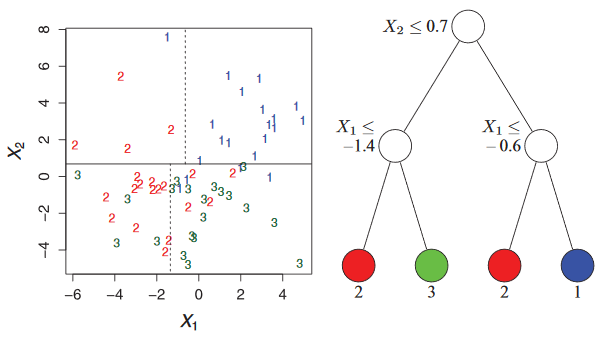
\includegraphics[scale=.52]{Partitioning}
	\caption{Left: Recursive partitioning of the $2$-dimensional space formed by $X_1$, $X_2$. Right: The resulting decision tree.}
	\label{Fig1}
\end{figure}	

An important question that we could ask regarding the construction of decision trees is how do we choose the features $X_i$, $i = 1,2,...,p$ in order to partition the $p$-dimensional space. It is reasonable that some features will provide better splits than others. The aim is to choose the feature that splits the parent node into two child nodes that are homogeneous or "pure", that is, each child node contains instances of only one class. This means that the feature we selected was able to discriminate well between the instances of the two classes. Each type of tree uses a different splitting criterion. C4.5 decision trees use the \textit{Gain Ratio} which is based on the calculation of entropy, whereas HDDT rely on \textit{Hellinger Distance}.

The gain ratio, also called information gain, measures the amount of information we gain by splitting the data using a specific feature. Features that result into "pure" or homogeneous splits yield higher values of gain ratio. Essentially, by increasing the gain ratio we achieve reduction in entropy. Entropy measures the impurity of an arbitrary collection of examples. It takes values in the interval $[0,1]$. High uncertainty corresponds to non-homogeneous splits in the two child nodes since we do not discriminate well between the two classes, which results to higher values of entropy. In formal notation, the entropy of a set $S$ is given by

\begin{equation*}
	I(S) = -\sum_{k = 1}^{T}p_k \ log_2(p_k)
\end{equation*}
where $T$ is the number of classes ($T=2$ for binary classification), and $p_k$, $k = 1,2,...,T$ indicates the proportion of instances in class $k$. Using a specific feature $X_i$ for splitting the $p$-dimensional space, by calculating the entropy of the parent node and the expected entropy of the resulted left and right child nodes, the gain ratio is calculated as 

\begin{equation*}
	G(feature) = I(S) - \sum_{v}^{}\frac{|S_v|}{|S|}I(S_v)
\end{equation*} 
where $S$ indicates the parent node and $S_v$ the child node. The result of Gain Ratio indicate the information we have gained by splitting the $p$-dimensional space using the selected feature. Using a greedy search, the feature that yields the highest gain ratio is chosen for the split.

\subsubsection{Splitting Criteria - Hellinger Distance}
HDDT use the Hellinger Distance as a splitting criterion for the construction of the tree. Hellinger Distance is a measure of distributional divergence \cite{Cieslak2008}. Let $P$ and $Q$ be two distributions of normalized frequencies of feature values across classes. If there is no distinction between $P$ and $Q$, that is, if $P$ and $Q$ overlap then the Hellinger Distance between the two distributions is equal to 0. In case $P$ and $Q$ are completely disjoint, the distance takes its  maximum value, $\sqrt{2}$. Hellinger Distance is utilized as a splitting criterion in the following way. Consider two class distributions $X_+$ and $X_-$ containing the instances of the positive and negative class, respectively. For a specific feature $X_i$, $i = 1,2,...,p$, the Hellinger Distance is given by 

\begin{equation*}
	d_H(X{_+},X{_-}) = \sqrt{\sum_{j = 1}^{p} \sqrt{\frac{|X{_{+j}}|}{|X{{_+}}|}} - 							\sqrt{\frac{|X{_{-j}}|}	{|X{{_-}}|}}}
\end{equation*}
where $j$ indicates the number of partitioned rectangles. For binary classification $j = 1,2$. $X_{+j}$ indicate the instances of the positive class in rectangle $j$, whereas $X_{+}$ represents all positive instances. The same holds for $X_{-j}$ and $X_{-}$ for the negative class. Due to the fact that the number of instances of the positive (minority) class in rectangle $j$ is conditioned with respect to all positive instances and because the prior probabilities do not explicitly appear in the distance calculation, Hellinger Distance is considered to be skew insensitive and well suited for classification in imbalanced data. A prior probability $P(+)$ is the probability for a randomly chosen instance to belong in the positive class. In the case of imbalanced data where the number of positive instances is less than the number of negatives, the prior probability $P(+)$ is very low. Hence, the fact that Hellinger Distance conditions the number of positive instances of rectangle $j$ to all positive instances of the data set without taking into account the prior probabilities, makes HDDT robust and well suited for classification in imbalanced data. The distance $d_H(X_{+},X_{-})$ is calculated for each feature. Using a greedy search, we choose the feature that returns the maximum distance.
 
\section{Data Sets and Software Tools}
\label{Sect.5}
\subsection{Data Sources}
Almost all link prediction works need to verify their methods on the collected datasets. The datasets are important for fairly reproducing and comparing different link prediction methods. Constructing and collecting the datasets is a time-consuming and labor-intensive work. That said, not all the datasets are publicly available to use and some of them are incomplete. Since the process of transforming the network to a data set requires the creation of two non-overlapping periods that simulate the formation of links between nodes from one period to the other, it is essential to consider networks that contain timestamps. We are interested in both directed and undirected networks. Nevertheless, we convert the former type to the latter. In all of our experiments, we consider unweighted networks.

%As mentioned in the sub-section Constructing Data Sets the dataset needs splitting into training sets and testing sets and to link-predict correctly our focus lies specifically on datasets with timestamps attached to each set of points this way we can easily check if a set exists in training set and test set given the dates of, for instances two authors previously worked together and might work together in the near future. 

%During scouting on the web for datasets we came across several useful datasets to which we think we can work with and produce some results with it. 

A summary of the size of nodes and edges, along with the length of the timespan of the social networks we consider can be found in \autoref{Table1}. We experiment with networks of different sizes and timespans in order to perform link prediction in different scenarios. We use three networks that come from the KONECT \footnote{\url{http://konect.uni-koblenz.de/networks/}} database. The first one is \texttt{UCIrvine} \cite{opsahl2009clustering}, a directed network containing sent messages between the users of an on-line community of students from the University of California, Irvine. Next, \texttt{Digg} \cite{de2009social} is a reply directed network of the social news website Digg where each node in the network is a user of the website, and each directed edge denotes that a user replied to another user. Furthermore, we use \texttt{Slashdot} \cite{gomez2008statistical}, a directed reply network of the technology website Slashdot, where nodes and edges represent users and replies, respectively. Moreover, we consider \texttt{RealityCall} \cite{eagle2006reality, nr} from Networks Repository \footnote{\url{http://networkrepository.com/ia-reality-call.php}}, which is an undirected network of mobile phone call events between a small set of core users at the Massachusetts Institute of Technology (MIT). The network also contains edges between users that do not belong in the small set of users, who called other individuals that were not actively monitored. Therefore, some sort of noise might exist in this network, since we do not have more information about the individuals outside of the small set of MIT users. Finally, we consider the directed \texttt{MathOverflow} network \cite{Paranjape:2017:MTN:3018661.3018731} that can be found on SNAP repository \footnote{\url{http://snap.stanford.edu/data/sx-mathoverflow.html}}. A node represents a user, and an edge indicates that user $u$ answered user's $v$ question on the website. All five networks are well suited for the link prediction problem. This is due to the fact that the nature of these networks is the interaction of individuals and we expect that connections taken place at time $t$ form a base for the connections that will form in the near future. Hence, we learn the patterns from interactions at time $[0,t]$, in order to predict future connections at $t' > t$.

\begin{table}
	\centering
	\scalebox{0.9}{
		\setlength\tabcolsep{3pt}
		\begin{tabular}{l c c c c c} 
			& \texttt{UC}  & \texttt{Digg} & \texttt{Slashdot} & \texttt{Reality} & \texttt{MathOver}\\ 
			\toprule
			Nodes & 1899 & 30398 & 51083 & 6809 & 21688 \\
			Edges & 59835 & 87627 & 140778 & 7680 & 107581 \\
			Timespan & 6 months & 16 days & 2 years & 4 months & 6.5 years
	\end{tabular}}
	\caption{Number of nodes, edges, and length of timespan for the 5 social networks.}
	\label{Table1}
\end{table}

%\begin{table}
%	\centering
%	\scalebox{0.9}{
%	\begin{tabular}{l c c c c c} 
%		& \texttt{UC}  & \texttt{Digg} & \texttt{Dublin} & \texttt{Reality} & \texttt{MathOver}\\ 
%		\toprule
%		Assortativity Coef. & -0.187 & 0.004 & 0.708 & ?? & ??\\
%		Clustering Coef. & 	5.68 & 0.56 & 1.06 & ?? & ?? \\
%		Mean degree & 63.017 & 5.7653 & 75 & ?? & ?? \\
%		Size Largest SCC & 1294 & 6746 & 335 & ?? & 3256\\
%		Size of nodes & 1899  & 30398 & 10972 & ?? & 21688 \\
%		Size of Edges & 59835  & 87627 & 44517 & ?? & 107581 \\
%		Timespan & ? & ? & ? & ? & ?
%	\end{tabular}}
%\end{table}

%Some of the sets we came across are either outdated or incomplete to so degree which was unusable. The social network datasets however are well maintained by some of the major datasets distributors such as Stanford University, this due that most of the researchers prefer to use these datasets. During the experimentation phase we noticed that some of sets contain noise\footnote{Noise make the networks inconsistent to the real-world networks.} and so a clean-up is required before usage. ~~And, when same metrics are compared on different datasets their performance ranks are usually not consistent or even various greatly~~. 
\subsection{Software Tools}
Although there are many link prediction metrics and methods proposed, only very few works open their source codes. Re-implementing methods and formulas to calculate predictors is a time-consuming process. Only few public tools try to integrate these metrics and methods such as \texttt{linkpred}\footnote{\url{https://github.com/rafguns/linkpred}} and \texttt{LPmade} \footnote{\url{https://github.com/rlichtenwalter/LPmade}} \cite{lichtenwalter2011lpmade} which both have a handful of link prediction metrics. \texttt{LPmade} is a cross-platform software solution that provides multi-core link prediction and related tasks and analysis \cite{lichtenwalter2011lpmade}. It is written in \texttt{C++} and therefore it is suited for handling very large networks. Unfortunately, compilation issues, and the lack of documentation and support prevented us from using the software. Hence, we used a \texttt{Python} library called \texttt{linkpred}. The main disadvantage of \texttt{linkpred} is that it is entirely written in \texttt{Python} and it can prove to be very slow for handling large networks.

\section{Experiments and Results}
\label{Sect.6}
\subsection{Experimental Setup}
We performed experiments in five social networks. The number of nodes, edges and the length of the timespan for each network can be found in \autoref{Table1}. All directed networks are converted to undirected, due to the limitations of \texttt{linkpred} library. The train set is constructed by considering the $n$-neighborhood size, where $n = 2$. For each network, we apply HDDT and C4.5 using the parameters proposed in \cite{Cieslak2012}. This setup consists of using bagging with 100 trees, un-collapsed, un-pruned, with Laplace smoothing at the leaves. Due to the huge size of the data sets, in order to be able to train decision trees but at the same time retain the imbalance, we under-sample the data sets to specified ratios. Specifically, we under-sample the larger networks \texttt{Digg, MathOverflow} and \texttt{SlashDot} to 1:10 ratio. Furthermore, we under-sample the smaller \texttt{UCIrvine} network to 1:10 and 1:60. From now on we will refer to them as \texttt{UCIrvine10} and \texttt{UCIrvine60}, respectively. Finally, due to the fact that \texttt{RealityCall} has only 56 positive instances, we can under-sample the data set to more extreme ratios. For \texttt{RealityCall} we use two versions, one under-sampled to 1:10 and the second to 1:600. We refer to them as \texttt{RealityCall10} and \texttt{RealityCall600}. In our experiments we also examine how the accuracy of the classifiers change when we move from smaller ratios of imbalance to larger ones. We perform 10-fold cross validation with stratified sampling for creating the train and test sets for each fold. A modified version of the WEKA software \cite{witten2016data} is used that contains the implementation of HDDT, which can be found in \url{https://www3.nd.edu/~dial/software/}. 

\subsection{Evaluation}
We evaluate the classifiers using the Receiver Operating Characteristic (ROC) curve and the Precision-Recall (PR) curve. The Area Under ROC (AUROC) metric is also provided, which quantifies the performance of a classifier. The main advantage of ROC and PR curve over single metrics such as accuracy is that they evaluate the classifier over all possible thresholds, whereas accuracy is specified only for a specific threshold. 

ROC curves contain the True Positive Rate (TPR), also called Recall on the $y$-axis and the False Positive Rate (FPR) on the $x$-axis. Recall is given by $\frac{TP}{TP + FN}$, where $TP$ and $FN$ indicate the \textit{True Positives} and \textit{False Negatives}, respectively. Thus, Recall gives the probability of classifying correctly a positive instance, given that it is positive. The $x$-axis represents the FPR, given by $\frac{FP}{FP + TN}$, where $FP$ indicates the \textit{False Positives}, and $TN$ the \textit{True Negatives}. A ROC curve closer to the upper left corner indicate a classifier that can accurately predict positive instances given that they belong to the positive class, for a low misclassification rate in the negative class, that is low FPR. The classifier that predicts each instance correctly has an AUROC value of 1. A classifier that is not able to discriminate between classes has an AUROC of 0.5 and its curve is a diagonal line at $f(x) = x$. Using ROC curves and the AUROC metric we can compare two or more classifiers. The one that has a curve closer the the upper left corner and thus greater AUROC value is considered to be a better classifier.

A supplementary metric to the ROC curve is the PR curve. The $y$-axis represents the precision, given by $\frac{TP}{TP + FP}$, that is the proportion of correctly classified positive instances over all instances that were predicted as positive. In other words, precision yields the probability of classifying a positive instance correctly, given that it was predicted positive. The $x$-axis represents the Recall. A classifier with a PR curve closer to the upper right corner is considered as a better classifier. 

\subsection{Calculated Features}
In all experiments we have calculated seven node-based and one path-based metric. Specifically, the node-based features consist of \textit{Common Neighbors, Jaccard Coefficient, Association Strength, Adamic Adar, Resource Allocation, Minimum Overlap}, and the \textit{NMeasure}. From path-based metrics we used \textit{Rooted pageRank}. Each measure is defined for a pair of nodes ${v,w} \in V_k$. The \textit{Common Neighbors} metric calculates the common neighbors of $v$ and $w$. Nodes with more common neighbors are more likely to connect in the future. \textit{Jaccard Coefficient} is a measure that returns the similarity of two sets. If we define the neighborhoods of $v$ and $w$ to be those two sets, the \text{Jaccard Coefficient} calculates how similar the neighborhoods are. Values closer to 1 indicate higher similarity. \textit{Association Strength, Minimum Overlap} and the \textit{NMeasure} are similar to \textit{Jaccard Coefficient}. Higher values indicate more similarity between the neighborhoods. The \textit{Adamic Adar} metric considers in its calculation the number of neighbors of all common neighbors of $v$ and $w$. The idea is that two nodes are more likely to connect in the future if their common neighbors have less number of neighbors. \textit{Resource Allocation} is similar to \textit{Adamic Adar} with the difference that common neighbors with larger number of neighbors are punished more heavily. Finally, \textit{Rooted pageRank} is a restricted random walk, where the output is the likelihood that a link will form between two nodes. An extensive comparison of different baseline predictors can be found in \cite{Liben-Nowell:2003:LPP:956863.956972}.

\subsection{Results}

\autoref{UCIrvine10} to \autoref{RealityCall600} illustrate the resulting ROC and PR curves for the five networks. C4.5 corresponds to the red curve, whereas HDDT to the black curve. Both types of trees exhibited similar performance in all networks. A more detailed comparison can be found in \autoref{Table2} where the AUROC metric is presented. HDDT out-performed C4.5 in \texttt{SlashDot} and \texttt{RealityCall10}, that is \texttt{RealityCall} under-sampled to 1:10 ratio. Note that the results of AUROC have not been tested for statistical significance as in the case of \cite{Cieslak2012}. That is, since the AUROC for both type of trees are very close to each other, the differences between them might be due to randomness.

It is clear that both classifiers perform from average to very good in the ROC space, while they perform poorly to average in the PR space, except in the case of \texttt{RealityCall10} where high precision can be observed. The poorest performance can be observed in \texttt{UCIrvine60} where the AUROC is about 0.77, and the highest precision is almost 0.25 which is achieved for low values of recall. Both classifiers performed better on \texttt{Digg} and \texttt{MathOverflow} with AUROC at about 0.81 and 0.8655 respectively. Nevertheless, precision is still relatively low for the different values of recall. For \texttt{SlashDot}, the resulting AUROC is about 0.9075, with a small improvement in precision. Both classifiers performed very good in \texttt{RealityCall10} network in the case of 1:10 ratio. Finally, in the more extreme case of 1:600, the recall of the ROC curve changes slightly, whereas the precision deteriorates significantly.

An insight that we can derive by examining the plots is that, the ROC curve seems to be insensitive as the imbalance of classes becomes larger. This is clear in \texttt{UCIrvine} and \texttt{RealityCall}. As we increased the imbalance from 1:10 to 1:60, and 1:10 to 1:600 respectively, we observe minor differences in ROC, while the results of PR differ significantly. The PR curve provides useful information as a supplementary metric to ROC. The use of PR curve is very important to consider as an evaluation of a classifier, a consideration that is not always taken into account in many studies that deal with imbalanced data.
% A second insight is that, in networks such as \texttt{SlashDot} and \texttt{RealityCall} where the results of both ROC and PR curve improve, HDDT outperforms C4.5. Hence, it might be the case that Hellinger Distance performs better in imbalanced data when there is not great overlapping of the positive and negative distributions.

The results of the ROC and PR curves indicate that both classifiers yield few \textit{FN} due to high recall, but a lot of \textit{FP} because of low precision. Thus, the probability of classifying an instance correctly as positive, given that it is positive is relatively high, but the probability of classifying an instance correctly as positive given that it was predicted as such, is relatively low. Whether or not the performance of a classifier is considered acceptable is usually domain specific. For example, when dealing with a terrorist network where the main focus is to not miss links that will form in the future, a metric such as recall would be more appropriate than precision. This is because high recall values will result to less \textit{FN}, that is, less instances of the positive class will be classified as negatives. In other cases where \textit{FP} are very important, the PR curve would be more informative.

By examining the top nodes of the resulting trees, we get an indication of which features were the most prominent in the construction of the tree. \autoref{feature_importance} illustrates those features for both HDDT and C4.5. \textit{Association Strength} was the most prominent feature in most networks. The features are displayed with respect to importance in descending order. The less important feature is \textit{Minimum Overlap}. 

\begin{table}
	\centering
	\scalebox{0.9}{
		\begin{tabular}{ c c c}
			& \textsc{HDDT} & \textsc{C4.5}\\
			\toprule
			\multirow{4}{*}{\texttt{UCIrvine10}} & Association Strength & Association Strength\\
			& Rooted pageRank & Rooted pageRank \\
			& NMeasure  & Resource Allocation\\
			& Resource Allocation & Minimum Overlap\\ 
			\midrule
			\multirow{4}{*}{\texttt{UCIrvine60}} & Association Strength & Association Strength\\
			& Rooted pageRank & Resource Allocation \\
			& Minimum Overlap  & Jaccard Coefficient\\
			& Resource Allocation & Common Neighbors\\ 
			\midrule
			\multirow{4}{*}{\texttt{Digg}} & Association Strength & Association Strength \\
			& Nmeasure & Miminum Overlap\\
			& Adamic Adar & Rooted pageRank\\
			%& & NMeasure\\
			\midrule
			\multirow{4}{*}{\texttt{MathOverflow}} & Adamic Adar & Common Neighbors \\
			& Association Strength & Association Strength\\
			& Resource Allocation & Rooted pageRank\\
			%& & Adamic Adar\\
			\midrule
			\multirow{5}{*}{\texttt{SlashDot}} & Association Strength & Association Strength\\
			& Common Neighbors & Common Neighbors\\
			& NMeasure & NMeasure\\
			& Adamic Adar & Rooted pageRank\\
			%& & Jaccard Coefficient\\
			\midrule
			\multirow{3}{*}{\texttt{RealityCall10}} & Association Strength & Association Strength\\
			& Adamic Adar & Jaccard coefficient\\
			& Jaccard Coefficient & Adamic Adar\\
			\midrule
			\multirow{3}{*}{\texttt{RealityCall600}} & Association Strength & Association Strength \\
			& Rooted pageRank & Adamic Adar\\
			& Adamic Adar & Rooted pageRank\\
			\midrule
	\end{tabular}}
	\caption{Most important features as indicated by the top nodes of the decision tree.}
	\label{feature_importance}
\end{table}
	
\begin{figure*}
	\begin{multicols}{2}
		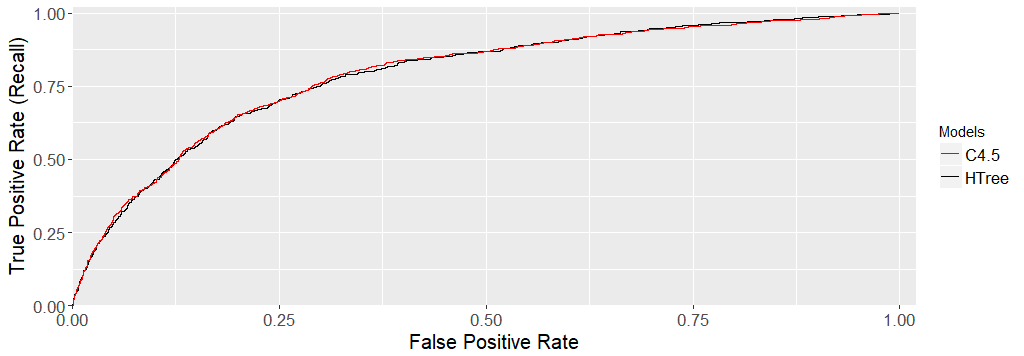
\includegraphics[width=\linewidth]{UC_Irvine_ROC_1_10}\par 
		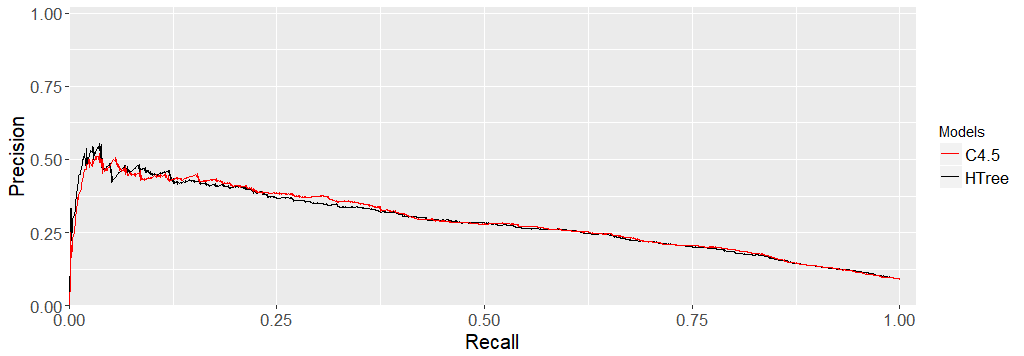
\includegraphics[width=\linewidth]{UC_Irvine_PR_1_10}\par 
	\end{multicols}
	\caption{\texttt{UCIrvine}, ratio 1:10}
	\label{UCIrvine10}
	\begin{multicols}{2}
		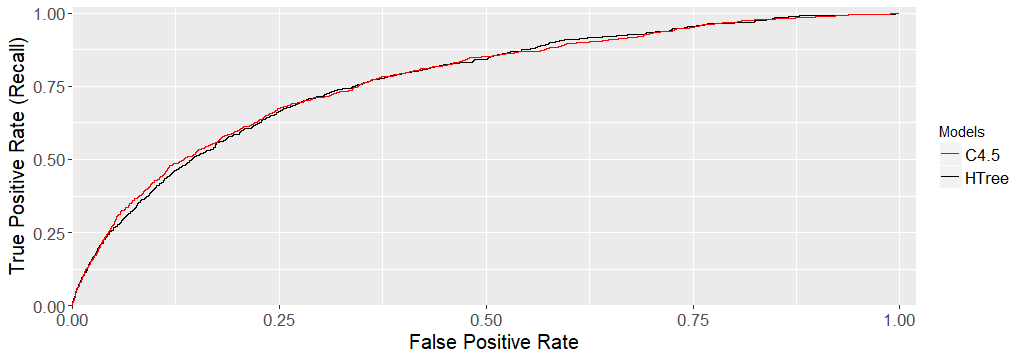
\includegraphics[width=\linewidth]{UC_Irvine_ROC_1_60}\par 
		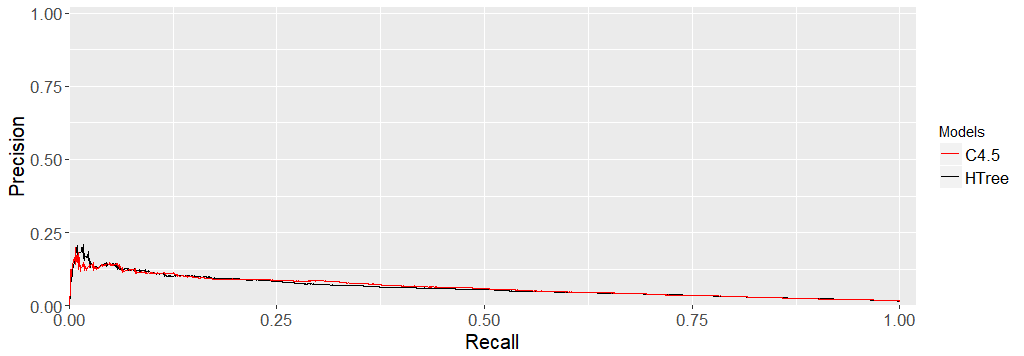
\includegraphics[width=\linewidth]{UC_Irvine_PR_1_60}\par 
	\end{multicols}
	\caption{\texttt{UCIrvine}, ratio 1:60}
	\label{UCIrvine60}
	\begin{multicols}{2}
		\includegraphics[width=\linewidth]{DiggNetwork_ROC}\par
		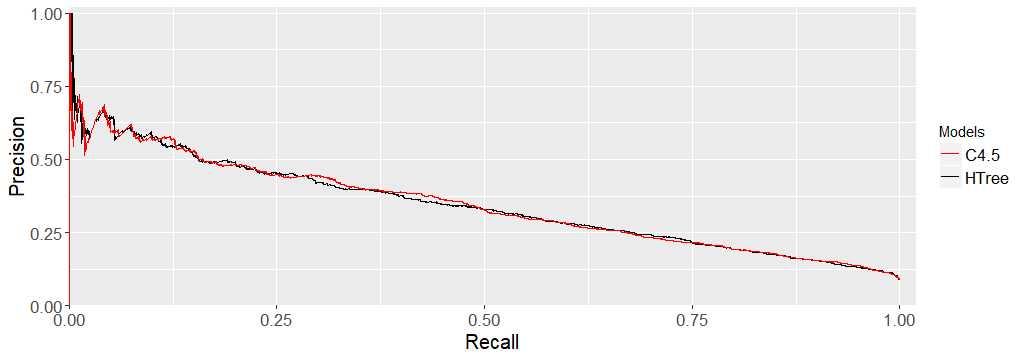
\includegraphics[width=\linewidth]{DiggNetwork_PR}\par
	\end{multicols}
	\caption{\texttt{Digg}, ratio 1:10}
	\label{Digg}
	\begin{multicols}{2}
		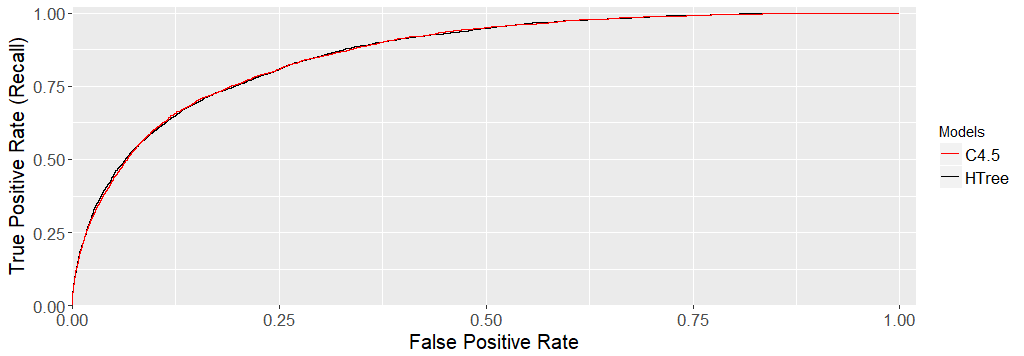
\includegraphics[width=\linewidth]{MathOverflow_ROC}\par
		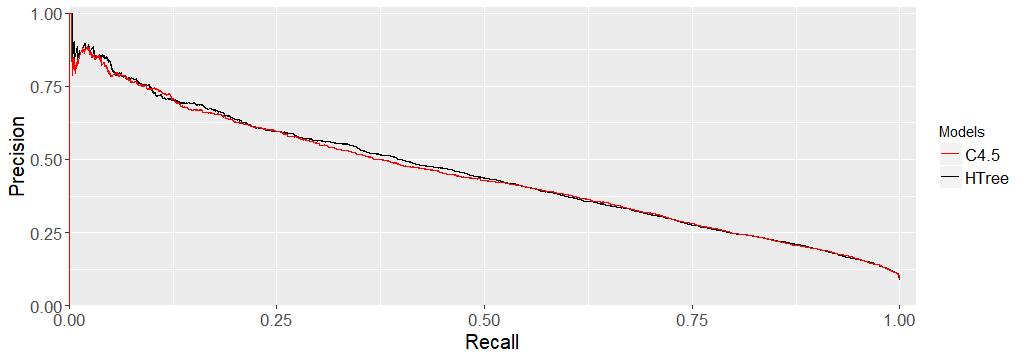
\includegraphics[width=\linewidth]{MathOverflow_PR}\par
	\end{multicols}
	\caption{\texttt{MathOverflow}, ratio 1:10}
	\label{MathOverflow}
	\begin{multicols}{2}
		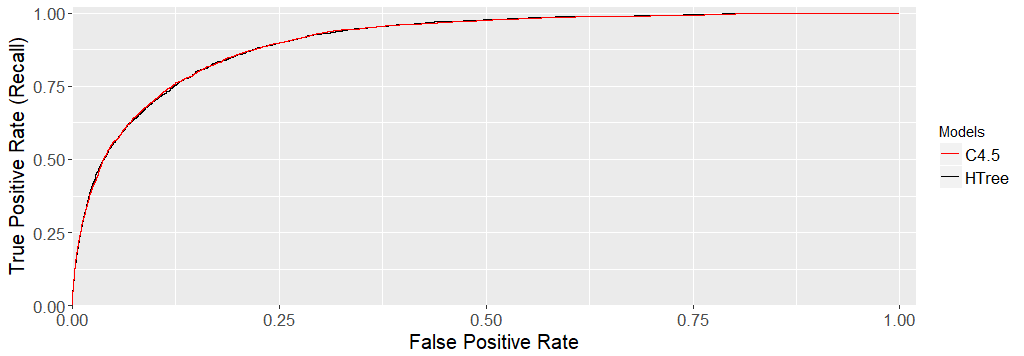
\includegraphics[width=\linewidth]{SlashDot_ROC}\par
		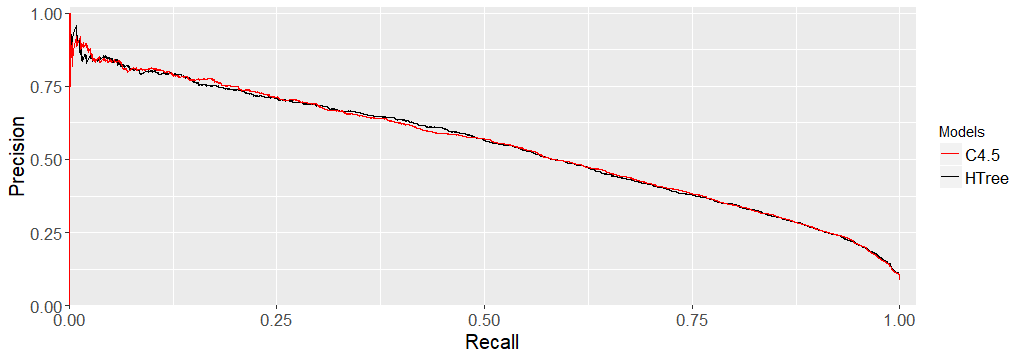
\includegraphics[width=\linewidth]{SlashDot_PR}\par
	\end{multicols}
	\caption{\texttt{SlashDot}, ratio 1:10}
	\label{SlashDot}
	\begin{multicols}{2}
		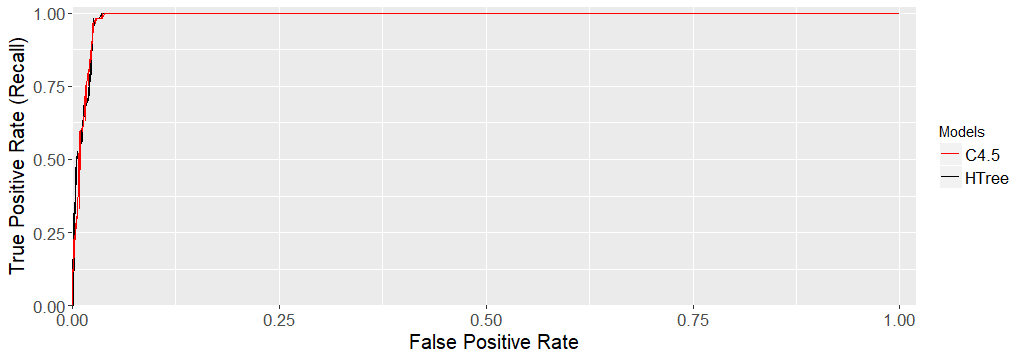
\includegraphics[width=\linewidth]{RealityMining_ROC_1_10}\par
		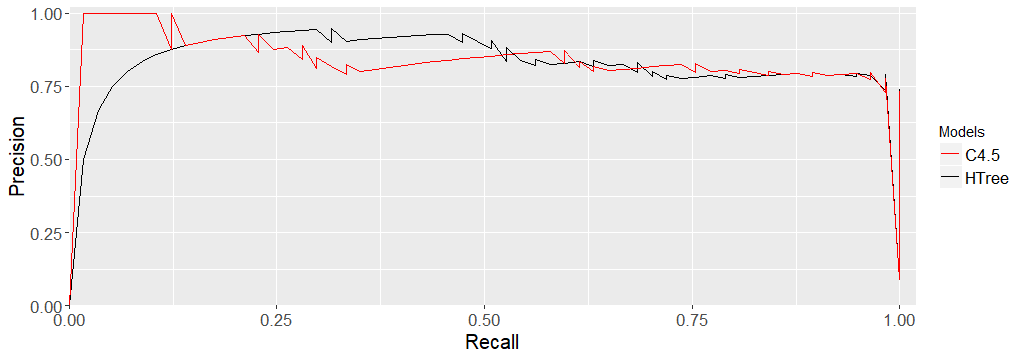
\includegraphics[width=\linewidth]{RealityMining_PR_1_10}\par
	\end{multicols}
	\caption{\texttt{RealityCall}, ratio 1:10}
	\label{RealityCall10}
\end{figure*}

\begin{figure*}
	\begin{multicols}{2}
	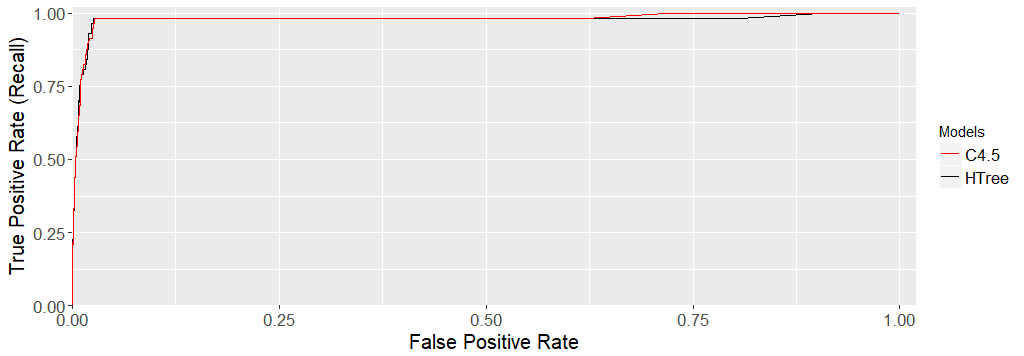
\includegraphics[width=\linewidth]{RealityMining_ROC_1_600}\par
	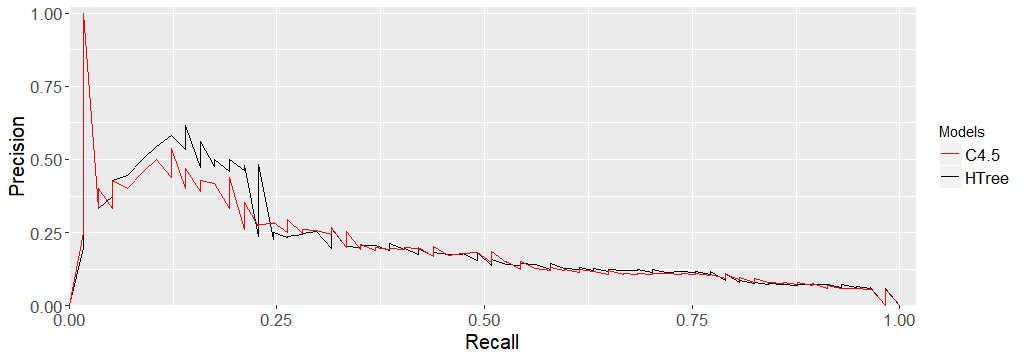
\includegraphics[width=\linewidth]{RealityMining_PR_1_600}\par
\end{multicols}
\caption{\texttt{RealityCall}, ratio 1:600}
\label{RealityCall600}
\end{figure*}

\begin{table}
	\centering
	\begin{tabular}{c c c}
		& HDDT & C4.5\\
		\toprule
		\texttt{UCIrvine10} & 0.7898 & \textbf{0.7912}\\
		\texttt{UCIrvine60} & 0.7712 & \textbf{0.7726}\\
		\texttt{Digg} & 0.8176 & \textbf{0.8185}\\
		\texttt{MathOverflow} & 0.8655 & 0.8655\\
		\texttt{SlashDot} & \textbf{0.9075} & 0.9074 \\
		\texttt{RealityCall10} & \textbf{0.9893} & 0.9888\\
		\texttt{RealityCall600} & 0.9783 & \textbf{0.9814}\\
	\end{tabular}
	\caption{AUROC for HDDT and C4.5}
	\label{Table2}
\end{table}

\section{Conclusions and Future Work}
\label{Sect.7}
In this paper we compared HDDT and C4.5 in seven imbalanced data sets constructed from five social networks. We evaluate both trees using ROC and PR curves. Both HDDT and C4.5 exhibited similar performance, with average to good performance on ROC space, and average to poor on the PR space. Thus, both classifiers yield high recall, but low precision. Additionally, as the class imbalance ratio increases, the precision gets lower, resulting to a larger number of \textit{FP}. On the other hand, the recall is not influenced significantly, that is the number of \textit{FN} does not increase. Regarding the baseline predictors that we used in our experiments, by examining the top nodes of the constructed trees we found that \textit{Associaton Strength} was the most important feature in six out of seven data sets. Our experiments were restricted to a number of chosen parameters such as the $n$-neighborhood size, where $n=2$. Furthermore, we under-sample the data sets into different ratios of imbalance in order to be able to train decision trees but at the same time retain the imbalance. Further research needs to be done in order to examine the effect of choosing different predictors and the number of $n$-size neighborhood. Finally, different under and over-sampling techniques could be used in order to improve the predictions of classifiers.

\bibliographystyle{abbrv}
\bibliography{snacspaper}  % sigproc.bib is the name of the Bibliography in this case

\end{document}
